

\chapter{介绍}

\section{概要}
这本书提出了关于灵长类动物前额叶皮层的基本功能如何进行定义。在本章中,我们将解释为什么我们在解决这个问题是采用了比较定义的方法。同时我们也解释了为什么我们关于基本功能的定义是依赖于理解大脑皮层区域之间的连接差异。因为我们的研究是基于细胞记录、影像激活和大脑病变这三种情况,本章解释了三种方法是如何相互关联的,并综合考虑了它们的优缺点。我们强调了一个成功的灵长类前额叶皮层理论的几个先决条件:该理论必须包含广泛的发现,该理论必须说明前额叶皮层的功能不同于其他皮层区域,该理论必须解释前额叶皮层带来的优势,该理论必须说明前额叶皮层作为一个整体的功能,且其功能必须是可测试的。

\section{介绍}
在这本书中,我们首先提出灵长类动物的前额叶PF皮层可以实现的基本功能:可以利用当前行为环境的信息,根据当前的生物的需求产生目标活动。PF皮层是如何执行这一功能以及它如何精准的执行功能是这本书的两个关键主题。当然,我们很清楚,很多书和文章都涉及这些主题,但这本书的不同之处在于还有另外两个问题:为什么前额叶皮层会理解做它所做的事情,以及它是如何做到的它要实现的事。
\par 
这些问题的出现是因为生物学需要针对问题做出两个方面的回答。比如说问,为什么在危险的情况下,心率会加速。一个答案是:当大脑检测到危险,并产生自主输出时起作用的生理机制等等。另一个答案是基于生物进化史,我们的大脑、心脏和循环系统保持原样并要维持它们所做的事情,生理学和系统发育学都会导致心跳加速。
\par 
Tinbergen阐述了这个概念,提出我们对任何生物系统应该思考的四个问题:它是如何进化的(系统发育)?;它如何促进健康(选择)?;它是如何发展的(个体发生)?;以及它是如何工作的(机制)?关于前额叶皮层的文章通常会处理最后两个问题,但很少会解决前两个问题。然而,我们在本书中认为这两个问题是理解前额叶皮层的关键。
\par 
当然,神经科学家可以说,他们对进化或健康不感兴趣。但我们认为他们这样做犯了一个策略错误。正如第二章所解释的那样,PF皮层的一些部分首先出现在早期灵长类动物中,其他部分则出现在灵长类动物的进化中。忽视这段历史,神经科学家会对前额叶皮层的研究失了一些重要的见解。
\par 
事实上,我们是类人猿的灵长类动物,是类人猿、人类和猴子的最后一个共同祖先的后代。我们看到的世界就像任何其他的类人猿一样,事通过一个中央凹看到的世界在精致的细节,像大多数类人猿一样是全彩的。其他种类的哺乳动物,甚至其他种类的灵长类动物,都缺乏这些视觉专门化。与其他哺乳动物相比,我们的嗅觉和味觉和听觉能力都不佳。但我们对这个世界的了解与其他哺乳动物不同——而且更有效。PF皮层不仅是理解我们如何做到这样做的关键,而且也是理解这是如何发生的关键。

\section{目的}
针对本文研究的两大主题,我们针对性的提出了五个目标,并在这本书中明确地说明了我们想要实现的目标。分别是:
\par 
  1.说明灵长类动物PF皮层是如何进化的,以及PF皮层给灵长类动物带来了什么优势。 
\par 2.说明灵长类动物的神经连接是如何定向到PF皮层,而不是其他大脑皮层区域来执行所需要实现的功能。 
\par 3.对灵长类动物PF皮层的基本功能提出一个具体的定义。
\par 4.在基本功能的定义下,解释当人们在执行复杂的认知任务时,大脑皮层产生的成像结果。
\par  5.告诉读者我们的定义与其他文献中的不同,以及我们该如何对其功能进行测试。
\par 
这些目标都很重要。我们考虑当忽略第一个问题会产生什么结果?为了实现这一点设想,我们需要了解不同哺乳动物物种的皮质区域之间的同源性。关于PF皮层功能定义的两种流行观点认为:PF皮层的基本功能是工作记忆或监测工作记忆中的项目(。这些功能被归因于PF皮层的一部分,正如第二章所解释的,这是专门在灵长类动物中进化的,而非灵长类哺乳动物的。
\par 
有人可能会认为,没有PF皮层这部分同源物的动物将会缺乏工作记忆或监测其内容物的能力。然而研究结果显示并非如此,例如老鼠可以学习径向分支迷宫任务。实验者用食物颗粒代替迷宫的八个分支,饥饿的老鼠只需全部访问一次分支,就可以来学习到收集颗粒的路径。老鼠可以学习分支迷宫任务的事实表明,它们可以记住和监测它们的哪条分支之前访问过。因此,一个全面的理论必须解释:为什么灵长类动物需要它们的PF皮层的某些部分来完成,其他哺乳动物在没有这些区域的同源物的情况下也可以学习和执行的任务。
\par
我们的第二个和第三个目标特别重要,因为它们是PF皮层处理任务的特定功能,与大脑的其他部分相比。如果灵长类动物的部分PF皮层进化出来了,我们需要了解这些区域可以做什么,而大脑的其他部分不能做什么。如果缺少这部分的分析,就破坏了其他几种理论。例如,工作记忆、全球工作空间理论。多重需求理论未能区分PF皮层和后顶叶皮层的作用,在该理论中这两个皮质区域都有助于这些功能。所以这三种理论都归因于PF皮层的功能,是因为其他区域也有作用。然而,理解灵长类动物PF皮层的关键:在于理解其功能与皮层的其他部分的不同。
\par
我们的第四个目标需要理解我们提出的PF皮层的基本功能是如何解释当人们执行复杂的认知任务时大脑产生的成像结果。大脑执行的任务如此之多,一个简单的叙述似乎没有希望。人们可能会问,一个简单的功能,无论多么基本,是如何解释复杂认知过程中的成像结果呢?
\par
我们的第五个也是最后一个目标似乎与其他目标不同,但它也同样重要。其他文献中的许多定义都很笼统,以致于它们永远无法被驳倒。举个例子,PF皮层的执行功能几乎没有提供什么可验证的假设,也没有论证是否有任何不涉及执行功能的重要行为。与一些关于PF皮层的理论不同,我们提出的观点应该很容易被反驳:人们只需要证明大脑的其他部分执行了我们提出的功能,或者灵长类动物的PF皮层没有执行这种功能。
\par
我们的五个目标决定了这本书的结构。第二章讨论了第一个目标:探索灵长类动物PF皮层的进化。第3-7章提出了第二个目标,那就是说明灵长类动物的神经连接是如何定向到PF皮层,而不是其他大脑皮层区域来执行所需要实现的功能。第三个目标是关于PF皮层作为一个整体的功能,因此第8章提出了这本书的定义。第9章通过检查人类脑成像文献来探讨第四个目标。第10章实现了我们的第五个也是最后一个目标,通过比较我们的定义和其他突出的想法和定义进行比较,以及提出如何对我们的定义进行测试。
\par
我们希望任何了解基本神经解剖学的神经科学家都能理解这本书,但我们不认为他们对PF皮层或用于研究研究PF皮层的方法有任何专业知识背景。因此,本章的其余部分提供了一些关于术语的背景材料和一些关键的方法要点。



\section{定义和术语}
\subsection{PF皮层定义}
甚至连专家有时也会松散地使用额叶这个词。当Teuber(1964)年提出“额叶功能之谜”时,他指的是前额叶皮层,而不是整个额叶皮层。在阿林和富尔顿(1936年)的一次演讲之后的讨论中,神经学家斯坦利·科布提出了以下抗议:
\par
我可以说一下这个命名法吗?这完全混淆了一些概念,这种误解主要是由于缺乏对术语的精确使用。当我在这里听作者和讨论者的交流时候,我听他们说额叶被切除了,意味着前三分之二被切除了。我听说运动区过去是三种不同的东西,运动前区域和锥体束同样松散地使用。这种口语化的表述可能很亲切,但不科学!
\par
我们把这些术语的划分带到心脏,所以我们区分了额叶皮质和额叶的运动区。我们只在指整个额叶或指额叶皮层的病变时使用额叶一词,这些病变可能侵犯或削弱了运动前区域。
\par
我们也大大区分了前额叶皮层的颗粒状部分和非颗粒状部分。大脑皮层的类型可以根据内部颗粒层,第4层的细胞体的数量和密度进行分类。颗粒状区域有一个明显的层;颗粒状区域有较少的细胞体浓缩成第4层。当然,这是过于简单化了,但也很有用。灵长类动物PF皮层的最大部分具有颗粒状的细胞结构,因此很多人称之为颗粒状的前额叶皮层 
\par
虽然这本书关注的是颗粒状PF皮层,但我们包括了PF皮层内的某些颗粒区域,正如我们的定义。在关于眼眶和内侧PF皮质的章节中,我们讨论了它们的颗粒状和非颗粒状部分。在这样做的时候,我们认为这两个区域的颗粒部分赋予灵长类动物的优势。

\begin{table}[htbp]
	\newcommand{\tabincell}[2]{\begin{tabular}{@{}#1@{}}#2\end{tabular}} %换行指令
	\centering
	\caption{人类和猕猴大脑中的前额叶区域( 括号里是区域号)}
	\renewcommand\arraystretch{1.5}	%设置表格内行间距
	\begin{tabular}{llll}
		\toprule 
		种类 &区域   &  人类  & 猕猴 \\
		\midrule
		\tabincell{c}{颗粒状 \\ 前额叶皮层}&尾部额叶&尾侧 (8)&精密 (8)\\
		&背内侧额叶 & 额上和内侧皮层 (9)  &额上和内侧皮层 (9)\\
		&侧区9&  额上侧 (9) &额上侧 (9) \\ 
		& 中外侧额叶&  额中回(46) & 主沟(46)\\
		&后外侧额叶 &  尾额中回(9/46) & 尾主沟(9/46)\\
		&腹侧额叶& 额下回(45,47)  & 下凸性(45,12)\\
		&颗粒轨道额叶 &眶面(11),延髓 (13),延髓 (14) &眶面(11),延髓 (13),延髓 (14) \\
		%
		%
		&极前额叶  &额杆 (10)   &额杆 (10) \\
		\midrule
		\tabincell{c}{非颗粒状 \\ 前额叶皮层}&内侧非颗粒状前额叶  & \tabincell{c}{前扣带回 (24)、边缘下 (25) \\边缘前 (32)} & \tabincell{c}{前扣带回 (24)、边缘下 (25) \\边缘前 (32)}\\
		&外侧非颗粒状前额叶 & 尾区13和14和非颗粒状岛叶皮质 & 尾区13和14和非颗粒状岛叶皮质\\
		\bottomrule
	\end{tabular}%
\end{table}%

\begin{table}[htbp]
	\newcommand{\tabincell}[2]{\begin{tabular}{@{}#1@{}}#2\end{tabular}} %换行指令
	\centering
	\caption{前额区组术语 ( 括号里是区域号)}
	\renewcommand\arraystretch{1.5}	%设置表格内行间距
	\begin{tabular}{ll}
		\toprule
		区域 & 组成部分 \\
		\midrule
		尾前额叶 & 区域 8,包括额叶视野 (FEF)?、后外侧前额叶(9/46区)?  \\
		背前额叶 & 中外侧前额叶(46区),外侧前额叶(9区)?,后外侧前额叶(9/46区)? \\
		内侧前额叶&边缘下区(25区),边缘前区(32区),扣带前部区(24区),内侧区9和极前区(10区)  \\
		眶前额叶 & 粒状和粒状眶皮层(11,13,14),粒状岛皮层  \\
		腹侧前额叶&12/47区和45区?,44区? \\
		横向前运动& 背侧和腹侧前运动区\\
		内侧前运动& 前辅助运动区(preSMA),辅助运动区(SMA),扣带运动区(CMAs)  \\
		运动前皮层& 外侧和内侧运动前区  \\
		\bottomrule
	\par?:可能包含在一个组中的区域\\
		\par a:人类极前部皮层的内侧部分。
	\end{tabular}%
\end{table}%


\par
表1.1列出了我们在PF皮层中包含的区域,表1.2给出了额叶区域的分组。书中使用的缩略语清单和词汇表分别列在第19页和第21页。在这些页面上放一个书签可能会很有用。


\subsection{PF皮层标记}
为了讨论灵长类动物的前皮层,我们需要采用一种命名惯例。如图1.1所示,von Bonin和Bailey(1947)用一个单一的名称来称呼PF皮质的大部分颗粒:FD区。那不符合我们的目的。尽管如此,我们展示了他们的地图,以表明颗粒状PF皮层具有足够的同质性,以至于von Bonin和Bailey将其大部分视为单个区域。

\begin{figure}[!htb]
	\centering
	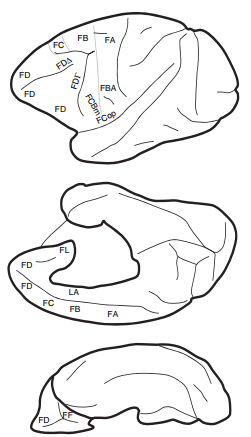
\includegraphics[width=0.5\linewidth]{image_pfc/Fig_1_1}
	\caption*{图1.1:von Bonin和Bailey绘制的猕猴皮层图(1947)。吻侧为左侧,顶部为侧位视图(背侧向上),中间为内侧视图(腹侧向上),底部为腹侧视图(侧侧向上)。请注意,von Bonin和Bailey将大部分前皮层指定为FD区,尽管他们识别了两个颗粒状区域:FF和FL。
		改编自von Bonin G, Bailey P. The Neocortex of Macaca Mulatta,©1947,伊利诺伊大学出版社。}
\end{figure}

\par
在冯·博宁和贝利的命名法中,一个区域名称的第一个字母代表一个脑叶:F代表额叶,P代表顶叶,T代表颞叶,O代表枕叶,L代表边缘。最后一个字母表示该瓣内的区域;例如,FA表示额叶区域A,与额叶区域B不同。
\par
布罗德曼简单地按照从大脑顶部到底部的顺序对他的区域进行编号,因为他在一系列水平的大脑区域中遇到了这些区域。所以4区就是从大脑顶部算起的第四个区域。有时很容易把冯·博宁和贝利的命名法和Brodmann命名法的两种命名联系起来:例如,区域FA与区域4相当接近。但有时,冯·博宁和贝利对大脑的看法与布罗德曼截然不同。
\par
如今,通常将这两种命名系统结合在一起,因为它们似乎对某些目的最有用。“布罗德曼区域”不再需要与布罗德曼自己描述的任何东西相对应,甚至不需要与他想象的任何东西相对应。
\par
除了前额叶皮层的颗粒区和颗粒区外,Brodmann、von Bonin和Bailey等人还发现了介于中间类型的皮层。颗粒区缺乏的第4层和颗粒区不缺乏的第四层有明显的不同,其他区域具有非颗粒细胞结构。这种类型的皮质有一个薄的,有时不连续的内部颗粒层。冯·博宁和贝利的区域额叶皮层划分有这个属性。一些区域,如FCBm(图1.1),有更多的中间属性,由字母组合指定。正如我们前面所说的,颗粒状和非颗粒状前额叶皮层之间的区别代表了一种有用的简化,而不是一种严格的二分法。Mackey和Petrides(2010)使用定量分析法证实,当人们沿着前额皮质的内侧或眶面朝上移动时,第4层变得更厚、更明显。
\par
在这本书中,我们使用了一个折中的名字组合。例如,我们使用字母TE和TEO来表示下颞叶皮层,这是由冯·博宁和贝利引入的。我们用6号区域作为运动前皮层,就像布罗德曼用的一样。我们使用了各种变体的大杂烩,例如,在Walker(1940)之后,极性PF皮层使用了10区。



\subsection{PF皮层细分}
关于前部皮层的细分还没有达成共识。正如刚才提到的,冯·博宁和贝利只区分出相对较少的额叶区域,但其他解剖学家已经发现了更多。例如,Petrides和Pandya生成了猕猴大脑的结构图(图1.2),通过识别更多的前额叶皮层细分来修改沃克定义的结构图。


\begin{figure}[!htb]
	\centering
	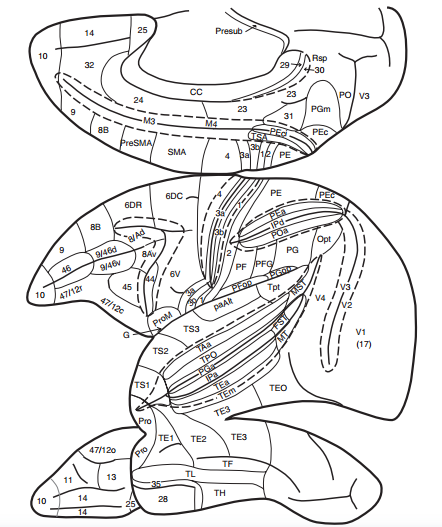
\includegraphics[width=0.5\linewidth]{image_pfc/Fig_1_2}
	\caption*{图1.2:由Petrides和Pandya绘制的猕猴皮层图(2007)。吻侧向左,内侧视图在顶部(腹侧向上),外侧视图在中间(背侧向上),底部腹侧视图(外侧向上)。缩写:CC,胼胝体;G,味觉皮层;Rsp,脾后皮质;Pro,前皮质,新皮质的变体;PreSMA,预辅助运动区;SMA,辅助运动区。区域的细分通常被指定为背(d或d)、吻(r或r)、腹(v或v)、眶(o)、眼(op)、内侧(m)、尾(c)或前(a)。猕猴吻侧前额叶皮层的传出关联通路。神经科学学报,27:11573-86,©2007,美国神经科学学会,已获许可。}
\end{figure}


\par
Petrides和Pandya(1995)也绘制了人类大脑皮层图(图1.3),与他们的猴子大脑皮层图非常吻合。然而,Carmichael和Price(1994)对大脑的看法不同。他们研究了猴子前脑皮层的眶面和内侧表面,发现了比Petrides和Pandya更多的细分,Öngür等人(2003)对人类大脑也做了同样的研究。

\par
神经解剖学家发表了相互矛盾的大脑前额叶皮层图,因为他们在是否以及在哪里检测到边界的问题上存在分歧。在大脑皮层的其他几个部分,神经生理学通过了地形图来帮助定义一个区域。在视觉、听觉和体感进行了区域划分,通常会定义一个区域及其边界。神经生理学对前额叶皮层没有这样的帮助。同样,不同区域的连接也帮助定义了大脑皮层。
\par
剩下的就是通过加入建筑学知识理解大脑皮层的区域划分,即通过选定的结构特征来识别区域的艺术,称之为皮层建筑学。当这些区域的特征是依赖于染色的细胞体时,这种做法被称为细胞结构学。当它们依赖于有髓鞘纤维的模式时,就称为髓结构学。这两种方法合在一起被统称为皮层建筑学。退一步说,这是一门不精确的科学。从本质上讲,皮层建筑学是一种非常高维的模式识别技能,需要多年才能掌握。因此,几十年来,一种客观、可靠、快速的标记边界的方法一直是皮层建筑学的圣杯。

\begin{figure}[!htb]
	\centering
	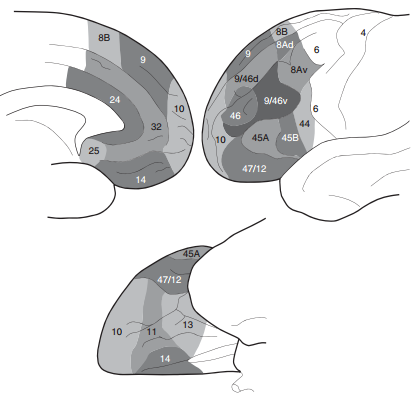
\includegraphics[width=0.5\linewidth]{image_pfc/Fig_1_3}
	\caption*{图1.3:Petrides和Pandya绘制的人类皮层图(1999)。在内侧视图(左上),吻侧在右侧;在侧视图(右上),吻侧在左侧;在腹侧视图中(底部),侧面是向上的。改编自Petrides M, Pandya DN。背外侧前额叶皮层:人类和猕猴大脑的细胞结构分析和皮质连接模式的比较。欧洲神经科学杂志,11:10 - 36,©1999,John Wiley和Sons,已获许可。}
\end{figure}


\par
Schleicher等人(1999)探索了一种他们称之为“观察者独立”的方法。他们的意思是,人类观察者不会检测到边界,而是由计算机来检测。细胞密度从最浅层(第1层)到最深层(第6层)变化。光密度测量可以反映这种变化,之间的差异反映了不同层中细胞类型和堆积密度的差异。沿着皮质进行这些测量,加入统计方法可以检测出在不同皮质区域之间划分边界的显著变化。因此,我们有希望有一天,我们将有一个完整的猕猴皮层地图基于观察者独立的方法,但目前我们还没有找到。

\par
即使可以精确可靠地建立区域边界,它们也可能不对应于功能细分。例如,在初级运动皮层- Brodmann命名法的4区和von Bonin和Bailey命名法的的FA区-其内侧和外侧的细胞结构不同,内侧的细胞体更大。但这种特性仅仅是因为内侧运动皮层控制腿部,轴突向脊髓下方延伸,有很大的细胞体。细胞结构上的差异并不对应于功能上的差异,而是涉及身体不同部位的差异。如果解剖学家在左脑前部皮层中发现了类似的差异,会将这两个区域标记为单独的区域。但是,这种区别可能很少或根本没有说明功能。

\par
。
鉴于在识别前额叶皮层的功能细分方面存在的问题和不一致,我们选择使用一般的描述性术语。图1.4显示了猕猴大脑的这些术语;图1.5显示了它们与沟和编号区域的关系。这种方法的优点是不与任何特定的划分图绑定,同时与大多数其他的命名划分图保持一致。



\subsection{约定和缩写}
我们的建议主要取决于 PF 皮层的连接解剖结构。 因此,当我们审查成像研究的结果时,我们有时会检查激活峰值的位置,以便将它们与我们对猴子同源区域的了解联系起来。为此,我们使用了程序 MRIcro,它采用报告的激活站点坐标并显示它位于关于脑回和脑沟地标的位置。 结果,我们的账户
大脑活动的定位有时与作者不同。 我们希望他们会原谅我们的冒昧。
\subsection{概括}
鉴于不同 PF 区域的标签种类繁多,我们建议读者参考表 1.1 和 1.2。本章中的表格和数字需要一个警告词。 很容易申请
与猕猴和人类大脑皮层的某些部分同名; 这十分的另一件事是确定这些区域是它们的共同名称所暗示的:从共同祖先继承的同系物。 第 2 章讨论了这个主题。
\par
\par






\section{指纹}
现在我们转向一个关键概念,这是我们第二和第三个目标的核心。一个成功的PF皮层理论不仅必须解释它能做什么,还必须解释为什么它本身就能做到这一点。为了实现这些目标,我们要依靠“指纹”。这个比喻来自齐尔斯和帕洛梅罗-加拉格尔(2001),他们用它来描述一个极性图,显示了大脑皮质区域中各种神经递质受体和转运体的密度。正如在法医学中一样,神经递质“指纹”具有基于许多特征的识别功能。帕辛汉姆等人(2002)称一个区域的整体连接模式称为其连接指纹,就像我们在这里所做的那样。
\subsection{连接指纹图谱}
关于大脑皮层联系的严肃研究始于潘迪亚和库伊珀斯(1969)和琼斯和鲍威尔(1970),并一直持续到今天。当然,随着这些方法变得更加敏感和可靠,研究结果也会发生变化,同时也有其他原因。
\par
例如,基底神经节的输出在不同时间单独针对辅助运动区(SMA);针对初级运动皮层(区域4)和运动前皮层(区域6);或针对其他区域,包括运动前前区(前SMA)、扣带运动区(CMA)和颗粒状PF皮层;麦克法兰。最近的证据表明,基底神经节的输出也延伸到顶叶(Clower et al. 2005)和颞叶(Middleton 。毫无疑问,公认的解剖结构有一天会再次改变,但现在我们要利用我们所拥有的。
\par
一个皮层区域的连接指纹具有重要的后果,因为它的连接限制了其功能。显然,如果一个大脑皮层区域没有接收到视觉输入,它就不能执行视觉功能。Passingham等人(2002)利用来自解剖数据库的数据绘制了PF皮层不同部分之间的连接图。这个数据库被称为椰子(http://www.cocomac.org/),它指的是猕猴的共同关系连接。在最新版本中,它包含了来自413项研究的数据,包括39,748个连接条目。
\par
通过使用这些连接数据,Passingham等人表明,每个PF区域都有一组独特的输入和输出。对于每个区域,他们用极坐标绘制了连接的强度。图1.6显示了两个连接指纹,一个用于背侧PF皮层(区域9),另一个用于眼眶PF皮层内侧(区域14)。周长显示与特征区域相连的区域,半径表示每个连接的主观强度从1到3。
\par
帕辛汉姆等人也使用了多维尺度来研究这些联系。如图1.7 A所示,多维尺度显示没有两个区域具有完全相同的连接模式。最近,Averbeck和Seo(2008)也使用Cocomac数据库绘制了不同PF区域的长期皮质皮质连接。他们证实,每个PF区域都有一个独特的连接模式。
\par
大脑的任何区域是孤立的,所以我们需要在整个PF皮层的背景下理解PF皮层的每个部分。因此,帕辛汉姆等人(2002年)继续使用层次聚类分析表明,在PF皮层内,人们可以识别出具有相似连接的区域簇。Averbeck和Seo(2008)使用了一种不同的技术来定义这样的集群,并得出了类似的结论。
\par
图1.7 B显示了PF皮层内的五个簇(Passingham et al. 2002)。与Averbeck和Seo(2008)的分析一样,它仅依赖于连接。然而,当人们将这些基于连接的集群与PF皮层中每个区域的位置信息结合起来时,就会出现一个略微不同的观点。出于这个原因,我们使用了一个与Price和Drevets(2010)提出的方案非常相似的方案。他们识别了PF皮层的五个部分:内侧、眶侧、尾侧、背侧和腹侧。第3-7章逐章考虑这五个区域,图1.8说明了它们。在大多数情况下,这些界限与PF皮层的传统观点一致。
\par
例如,图1.7 A支持在猕猴的内侧PF皮层中包含极性PF皮层。每个区域构成了一个更大的区域网络的一部分,包括运动前、顶叶、颞叶和海马皮层。
\par
关于广泛的分布式神经网络的发现提出了一个挑战,这与我们的第二个和第三个目标有关。仅仅在一个网络中放置一个PF区域是不够的,我们还需要说明该区域与同一网络中的其他区域有什么不同。例如,包括中外侧PF皮层(46区)以及后顶叶皮层的几个部分的神经网络。这两个网络部分的病变对行为有显著不同的影响。
\par
延迟交替任务的经典版本要求猴子学会选择一个食物在一次试验中——选择左边的井,在下一个试验中选择右边的食物井,以此类推,从而在另一个试验中交替。有中外侧PF皮层(46区)损伤的猴子无法重新学习这项任务,但后顶叶皮层的损伤没有影响(Ettlinger et al. 1966)。解释肯定是,虽然中外侧PF皮层和后顶叶区域有许多共同的连接,特别是彼此之间,但它们并不共享所有的连接。每个区域的连接指纹都指向了重要的差异。
\subsection{生理指纹图谱}
一个区域的连接指纹显示了该区域的约束和功能。通过类推,帕辛厄姆等人(2002)引入了功能指纹的概念。他们用生理数据说明了这些特性,所以我们在这里使用生理指纹这个短语。对于一组数据,他们绘制了细胞活动的五种特性: (1)听觉或视觉反应;(2)本体感觉或皮肤反应;(3)类似肌肉的活动模式;(4)活动与运动的时间相关性;(5)持续的延迟期活动。
\par
图1.9 C显示,SMA和腹侧前运动皮层在不同的细胞类别中出现的相对频率有所不同。例如,SMA中有更高比例的细胞有躯体感觉反应。图中还显示了这两个区域的连接指纹的不同(图1.9 A和B)。
\par
对于第二个数据集,Passingham等人(2002年)绘制了细胞对基于记忆或基于视觉线索的运动序列的偏好( Mushiake等人,1991年)。图1.10中的直方图显示了SMA和运动前皮层的结果,活动分类从1到7。第一类细胞对视觉任务具有完全的特异性;第七类的细胞对记忆引导任务有完全的特异性。
\par
四种活动的分类表明它们在统计上是相等的活动。SMA在记忆引导任务中表现出活动的优势,而外侧运动前皮层则表现出相反的偏差。
\par
我们还以生理指纹的形式绘制了这些数据。图1.10顶部的极坐标图显示了与下面的柱状图相同的数据,单元类围绕周长绘制,每个类沿半径的比例绘制。


\subsection{行为指纹}
到目前为止,我们已经暗示,为了理解PF皮层,我们需要进行比较:连接指纹,比较解剖特性和生理指纹比较细胞活动。对行为的理解也能从比较中学到好处。然而,关于PF皮层的神经心理学文献通常只强调一些行为任务。截至2011年,至少有162篇论文出现在PF皮层损伤的猴子的延迟反应任务上,其中许多论文只处理了这一项任务。
\par
这种重点有其优点。例如,它允许在同一任务上进行行为、生理、成像和药理学实验。但是,对一个或几个任务的狭隘关注可能会产生对PF皮层功能的扭曲看法。在第5章和第6章中,我们解释了为什么延迟反应任务及其近亲,即延迟交替任务,会产生这种扭曲。这些任务的结果得出结论,PF皮层主要在工作记忆,如果不是完全在工作记忆。第10章解释了为什么我们拒绝PF皮层的理论。但是人们不需要知道为什么这样做就能认识到仅仅依赖几个任务的问题。根据两个任务得出结论,PF皮层在工作记忆中的作用,就像在参观了史密斯奶奶的两个小丛苹果后,得出所有成熟的苹果都是绿色的结论。
\par
我们并不质疑灵长类动物PF皮层的损伤会对这些任务的学习和执行造成严重和持久的损害,或者一些成熟的苹果是绿色的。灵长类动物的PF皮层一定有什么东西让它对这些任务的表现。但它需要进行任务之间的比较才能理解它是什么。因此,除了前面讨论的连接指纹和生理指纹外,我们还需要行为指纹,其中包括对不同任务之间的损伤效应的比较。我们需要了解患有PF损伤的猴子表现出损伤的广泛任务。

\subsection{总结}
一个区域的连接指纹限制了它能做什么。生理和行为指纹提供了对这种功能的见解。太多的关于PF皮层的理论是从一个或几个任务的发现中发展起来的。在第10章中,我们将我们所谓的通用性测试应用到PF皮层的理论中,即检验它们是否能够解释激发它们的任务之外的数据。为了确定灵长类动物PF皮层的基本功能,我们需要依赖于广泛的发现,以连接、生理和行为指纹为特征。

\section{损伤和激活}
鉴于成像技术使研究完整的人类大脑成为可能,人们可能会认为,当我们试图理解PF皮层时,我们不再需要吸引大脑损伤的影响。毕竟,作为应用于人类受试者,影像学比病变研究有两大优势。首先,激活的峰值位于灰质,而在患者的病变往往损害潜在的白质。第二,这些山峰可以,而且经常可以,位于特定的区域内。相比之下,患者的病变通常包括许多不同的区域。
\par
鉴于这些优势,读者可能会想知道为什么我们如此重视病变的影响。我们这样做是因为对某一区域的活动或激活的观察并没有告诉我们,受试者在没有该区域的情况下无法执行任务。以Price等人(1999)的成像研究为例。他们的研究对象看到了一系列的照片,其中一张被指定为目标。在每次试验中,他们必须从两张照片中选择哪一张与目标相关。例如,当他们面对一把钳子时,他们必须选择一个扳手而不是一个锯子。钳子和扳手放在一起,因为它们能抓住东西,而把它们放在一起需要语义分类。
\par
激活发生在三个部位:左侧颞叶中皮层、左侧颞叶下皮层和左侧腹侧PF皮层。但Price等人也扫描了一名左腹侧PF皮质完全病变的患者。患者仍然可以执行这项任务,即使在任何剩余的PF皮层中都没有被激活。因此,我们可以得出结论,左腹侧PF皮层对执行语义分类任务并不是必需的,即使它在执行任务的过程中显示出激活。我们还可以推断,颞中层和颞下皮层足以完成任务,而腹侧PF皮层没有任何贡献。我们只能通过结合影像学和研究病变的影响来得出这个结论。
\par
不幸的是,这种方法,因为很难找到只有一个区域病变的患者。虽然暂时性病变,如重复经颅磁刺激(rTMS)引起的这些方法,为寻找特定病变的患者提供了一个有用的选择,这种方法也有严重的局限性。人类的大部分皮层埋在沟深处,刺激不能选择性地到达它。此外,刺激效应的精确解剖边界尚不清楚。
\par
因此,我们严重依赖于猴子的大脑皮质损伤的影响。通过使用选择性的手术技术,人们可以单独切除皮质,同时保留下面的白质完整。人们可以选择性地去除特定区域,特别是沟提供有用指导的地方。病变的边界稍后可以通过合理的准确性进行评估。作为一种选择,人们可以选择性地、暂时地灭活一个区域。
\par
由于其更高的解剖精度,我们严重依赖于猴子的实验结果来理解损伤的影响。这并不意味着我们完全忽略了对患者的研究结果。这些观察结果可以在若干方面发挥作用。例如,脑损伤的行为影响可能很难在猴子身上进行解释,而在人类患者身上进行的研究则可以帮助解决这些困难。
\par
以两个匹配的任务为例。在延迟的样本匹配任务中,猴子首先看到一个对象(样本),在延迟一段时间后,它们必须从两个匹配样本的对象中选择一个。我们称之为匹配规则。在延迟的非匹配到样本的任务上,他们需要选择另一个对象:非匹配规则。
\par
假设有PF皮层损伤的猴子在这些任务上表现出损伤。这可能是他们不能记住样本,或者不能识别出两个相同或不同的对象,也可能是他们不再知道任务规则。研究PF皮质病变患者的一个优点是,我们可以告诉他们规则,然后检查他们是否知道。如果他们不能正常地执行任务,但可以告诉实验者规则,这就可以作为他们忘记了样本或在识别两个物体匹配方面存在问题的证据。
\par
这个示例还指出了依赖于任务名称的危险。匹配和非匹配的任务也被称为“识别记忆任务”。如果猴子只能以一种方式执行这些任务,这个名字就可以了:通过记住和识别物体。不幸的是,就像猴子研究中使用的许多任务一样,这些任务有几种替代策略。猴子可以根据识别度、熟悉度或近因性来选择一个物体,这取决于每个实验的细节,有时实验者并不知道猴子是如何执行任务的。具体的比较条件可以区分这些策略,但它们并不总是被使用。类似地,我们稍后将讨论涉及所谓的自我分配任务的实验。事实上,是受试者还是实验者产生这个顺序并不重要(佩特里德斯1995),所以如果从字面上看,这个名字可能会产生误导。
\par
然而,只要人们要仔细解释病变的影响,这种方法仍然提供了关于一个区域的功能的一些最重要的证据。金标准被称为功能的双解离。这意味着一个区域的病变会损害一项任务的表现,而不损害另一个任务的表现,以及某些区域的病变其他区域对这两个任务都有相反的效果。例如,腹侧PF皮层的损伤会破坏猴子执行一种策略任务的能力(Baxter et al. 2009),而眼眶PF皮层的损伤则不会(Baxter et al. 2007)。相比之下,眶部PF皮质损伤会破坏贬值任务的表现(Izquierdo等,2004年),而腹侧PF皮质损伤不会(Baxter等,2009年)。第4章和第7章详细地解释了这些任务及其含义,但即使没有这些细节,我们也可以看到,这些结果建立了某种功能的双重分离。
\par
尽管有这些和其他几个例子,Gaffan指出,这类物质的双重分离不如通常认为的PF皮层常见。Wilson等人(2010)强调,从整体上影响PF皮层的操作通常比主要影响部分皮层的操作产生更大的影响。这些发现支持了PF皮层作为一个整体起作用的观点,第8章就讨论了这个主题。
\subsection{总结}
在一个由成像实验主导的领域,许多神经科学家似乎认为,在考虑皮质区域的功能时,对病变效应的理解并很少。我们使用了影像文献中的一个例子来反驳这一观点:影像激活显示了信息处理的内容,但它们没有像病变研究那样在某些任务或功能中发挥必要的作用。
\section{损伤和活动}
前一节对比了病变和影像学方法;本节对比了病变和细胞记录的方法。这两种方法告诉了我们不同的事情。因为它们这样做了,病变的影响似乎并不总是与发生在同一区域的细胞活动相匹配。我们在前面讨论了一个例子。在猴子中,中外侧PF皮层(46区)和后顶叶皮层的损伤有不同的影响,尽管这两个区域相互联系,在各种任务中具有相似的细胞活动。我们之前提到过,中外侧PF皮质损伤的猴子无法学习延迟交替任务,而后顶叶皮质损伤较大的猴子则能正常执行该任务。然而,中外侧PF皮层和后顶叶皮层细胞在延迟期间都表现出持续的活动,这是猴子必须记住执行任务所需的信息的一段间隔。因此,细胞活动和损伤效应在中外侧PF皮层相当匹配(持续活动和损伤效应),而在后顶叶皮层则不是( 持续活动,但没有损伤效应)。
\par
另一个例子是,考虑运动前区域的内侧和外侧组,它们有广泛的相互联系(Luppino et al. 1993)。内侧区域的病变严重破坏了自我产生的运动,定义为没有视觉线索提示的运动。外侧的运动前区病变没有这种影响(Thaler et al. 1995);它们反而会影响视觉提示的运动。考虑到内侧和外侧运动前区的许多细胞是否能排出运动,这可能是视觉提示的还是自我引导的?图1.10显示,这两个区域的许多细胞都属于第四类,这表明两种引导形式的活动在统计上是相同的。其他细胞也表现出偏见,但它们在这两项任务中仍然有显著的活动。
\par
为了回答这个问题,我们需要认识到,损伤会告诉我们,在没有损伤区域的情况下,大脑的其他区域可以做什么或不能做什么。病变不仅消除了受损区域的计算资源,还消除了对其他区域的输入,以及其他影响。在完整的大脑中,当动物进行自我引导运动时,外侧运动前皮层的细胞表现出活动增加(图1.10中的第5至7类)。因此,人们可能会认为,在没有内侧运动前区的情况下,外侧运动前区可以接管自我产生的运动。但假设这些细胞从内侧前运动区获得输入,这些连接产生了第5到第7类细胞。然后,在受损的动物中,这些细胞将不再具有与正常动物相同的特性。因此,在没有内侧前运动区的情况下,外侧运动前区不能“接管”自我引导的运动。
\par
这种思路解释了一个原因,即某些区域可以显示出某些行为的活动,即使它们在这些行为中没有发挥必要的作用。类似的原理也适用于PF皮层。在一个典型的条件视觉运动任务中,一张图片指示猴子做出一种反应,而另一张图片指示出不同的反应。细胞在中外侧PF皮层和腹侧PF皮层区域编码这些图像反应映射(Asaad et al. 1998)。然而,这两个区域的病变的影响是不同的。腹侧PF皮层的损伤在这项任务上产生严重的损伤(Wang et al. 2000),但中外侧PF皮层的损伤只有轻微的影响(Petrides 1987)。我们可以用第一个例子一样的方式调和这些发现。腹侧PF皮层的损伤切断了从颞下皮层到中外侧PF皮层的大部分输入(Ungerleider,etal.1989;韦伯斯特等,1994),因此中外侧PF皮层不能“接管”该功能。
\par
由于病变和细胞记录方法的优缺点,我们需要比较细胞活动与脑损伤的影响,以便从这两种信息来源中获得最大的好处。
\par
书中不时出现的另一种活动涉及到皮质内的微刺激。这种方法通过用于研究单细胞活性的相同类型的电极引入电流。因此,它至少在数百个细胞中同步产生活动。与正常发生的放电的比较是复杂的,但该方法提供了有用的信息,假设它大致模拟正常活动。
\subsection{总结}
大脑皮质损伤的影响并不总是像人们可能预期的那样与细胞活动相匹配。在本节中,我们已经解释了发生这些明显的不匹配的一个原因。病变效应和细胞活动都取决于一个区域的连接,但其方式不同。细胞活动反映了通过连接接收信息或在一个区域内的信息处理。这些结果反映了神经相关性而损伤效应则揭示了一个区域对该行为的必要贡献。


\section{活动和激活}
在后面的章节中,我们自由地将关于大脑区域激活的讨论与关于细胞活动的发现相结合。然而,这种组合需要谨慎使用,原因有两个:血管伪影和细胞活性和成像激活之间关系的不确定性。
\par
首先,血氧水平依赖性(BOLD)信号是一种血管信号,因此它对大动脉的位置很敏感。BOLD信号也可能被静脉和静脉流出物的位置所污染(Turner 2002)。由于这些原因,其中,BOLD信号的峰值与潜在大脑活动的位置只有非常粗略的空间对应关系(Kim et al. 2004)。
\par
其次,我们对成像激活和细胞活动之间的关系所知甚少。对猴子的成像和细胞活动进行直接比较会有帮助,但要对理解PF皮层有任何价值,这种比较必须对一个稀疏编码的网络进行比较。在稀疏编码的网络中,附近的细胞具有不同的属性;在一个密集编码的网络中,大多数细胞做同样的事情。由于这种相对的同质性,来自密集编码网络的结果,如感觉或运动区域,有潜在的误导性。我们只有少量关于猴子稀疏编码网络的成像数据,如PF皮层或海马体(Nakahara et al.,2002;Orban等,2004)。因此,我们必须运用一般的原则。
\par
成像实验测量了BOLD信号。在没有动作电位的情况下,BOLD响应可以发生(Logothetis 2002),当峰值活动没有发生时,BOLD信号可以在不同的实验条件下有所不同。例如,Maier等人(2008)研究了猴子初级视觉皮层中的BOLD激活和单细胞活动。他们使用了一种叫做广义闪光抑制的知觉操作。当移动的点突然出现在视觉目标刺激周围时,它们会抑制对目标刺激的感知。抑制性刺激并不影响视觉皮层的单细胞活动,但它们确实影响了BOLD信号。这一发现表明,BOLD信号对调节效应很敏感(Logothetis 2008),这可能是由抑制性突触输入或低于驱动细胞活性阈值的兴奋性输入介导的。
\par
一个研究得特别充分的例子涉及到小脑。虽然突触激活与BOLD信号密切相关,但其输出神经元浦肯野细胞的活动却不相关(Thomsen et al. 2004)。向浦肯野细胞的突触输入,而不是浦肯野细胞的活动,驱动BOLD信号(Gold 和 Lauritzen 2002)。氧消耗与浦肯野细胞的两种主要输入诱导的局部场电位线性增加:攀爬纤维(Offenhauser et al. 2005)和平行纤维(Thomsen et al. 2009),这些电位反映的是突触输入,而不是浦肯野细胞的放电活动。
\par
因此,大多数证据支持这样的结论,即在成像研究中测量的信号并不直接反映神经元的活动,而是反映了突触的输入。有时,净突触输入(激活)与神经元活动相关,但通常它不是。由于这个原因,我们在整本书中将细胞活动区分为区域激活。我们通过激活来反映突触的影响,而不是单个细胞的放电率(Logothetis 2002)。
\subsection{ 元分析}
我们之前提到过,在解释病变效应时过度依赖一项或几个任务的危险。同样的警告也适用于细胞记录和成像。在一项经常被引用的研究中(Funahashi et al. 1989),猴子注视着一个中心光点,一个提示出现在八个地方中的一个。在一段延迟后,一个“去”提示触发了对提示位置的扫视运动。在延迟期具有显著活性的细胞中,百分之八十的编码了提示的位置。可以理解的是,许多神经科学家认为这一结果与细胞编码记忆位置的想法是一致的。
\par
但是,仅基于一项任务就得出这个结论是危险的。细胞活动在一定程度上取决于猴子的训练历史。例如,弗里德曼等人(2006)训练猴子区分猫和狗的照片。他们发现,对训练中使用的方向的刺激具有更强的选择性。这一发现并不令人惊讶,因为动物(和它们的大脑皮层)从经验中学习。
\par
考虑到这一原则,富桥等人(1989)的结果为他们的解释提供的支持比他们想象的要少。如果我们只研究一个简单的空间记忆任务中的细胞活动,那就好像有许多细胞编码记忆的位置。
\par
但我们只能通过比较在其他任务上的细胞活动来测试这种印象。例如,延迟期间的细胞活动可能反映了猴子关注的地方以及它们记得的地方。因此,列别捷夫等人(2004)训练猴子记住一个地点和去其他地方。在对一个位置有选择性的PF细胞中,百分之六十一仅编码参与位置,排除了在记忆中的作用。只有百分之十六的细胞单独编码了记忆中的位置,其余的细胞具有混合特性。只有在不同任务之间的比较才能表明,在空间记忆方面对神经元活动的解释在很大程度上是错误的。
\par
在第8章和第9章中,我们通过统计许多任务的结果来认识到这种比较的重要性。表8.1显示了猴子的病变效应的汇编,表8.2显示了细胞活性特性的选择。表9.10对人的成像激活做了类似的操作。我们只能通过考虑广泛任务的结果,得出关于PF皮层的基本功能的结论。
\par
这种方法类似于成像文献中常用的方法。因为结果可以在一个共同的解剖坐标系中报告,所以可以执行元分析,其中涉及到来自导致一个区域激活的任务的数据的合成。荟萃分析是由另一个名字的生理指纹。
\subsection{总结}
虽然第3-7章没有使用极坐标图来说明连接、生理或行为指纹,但它们通过更传统的方法传达了相同的原则。对于神经解剖学的数据,他们在猴子大脑的地图上显示了一个特定区域的连接。他们强调,理解PF皮层需要比较不同大脑区域之间的连接( 连接指纹),以及比较损伤效应( 行为指纹),以及各种任务的活动和激活( 生理指纹)。虽然我们在序言中承认了樱桃挑选的数据,但我们希望读者会同意,我们已经尝试挑选了很多樱桃。
\par
本节对比了细胞记录和成像结果。和所有的方法一样,成像也有局限性。但与对细胞活性的研究相比,它至少有三个主要的优势:
\par 1.成像可以同时测量大脑的大部分区域。
\par 2.BOLD信号的峰值位置可能反映了一种特定功能类型的信号的峰值密度,而细胞记录将检测到一种活动类型发生的任何地方。
\par 3.BOLD信号似乎特别很好地反映了同步激活。例如,Parkes等人(2006),结合脑电图(EEG)和功能成像,发现同步性和激活密切相关。在低频范围内,BOLD信号与场电位之间的关系最接近(Kayser et al. 2004)。
\par 然而,细胞记录比成像记录有一些优势。它直接显示了一个区域的信息处理元素的编码。即使在成像实验中无法检测到不同的、混合的神经元种群,它也可以显示出不同的特性,这对于像PF皮层这样的稀疏编码的神经网络尤为重要。最后,细胞记录可以区分活动的增加和减少,而成像则不能。(成像可以区分激活的增加和减少,但不能区分活动。)例如,对成像文献的讨论很少指出,例如,激活的增加可能反映了对一个区域输出的抑制,这对于稀疏编码的网络尤其如此。

\section{结论}
这本书采用了一种比较的方法来提出一个关于灵长类动物PF皮层的基本功能的建议。它有五个明确的目标:描述PF皮层的优势,说其连接导致其独特的功能,考虑它是如何作为一个整体,占激活在人类认知任务,并解释我们的建议不同于别人的文献以及如何测试。
\par
为了实现第一个目标,第二章比较了PF皮层的物种多样性,生存和灭绝。为了实现第二个目标,第3-7章都以总结开始PF皮层的一个主要部分的连接。每一章的最后都是关于该部分的功能的简短但具体的建议。为了实现第三个目标,第8章建立在第3-7章的建议的基础上,提出了一个关于PF皮层作为一个整体的基本功能的建议。为了实现第四个目标,第9章解释了我们如何解释当人们执行复杂的认知任务时的成像激活。最后,对于第五个目标,第10章将我们的建议与文献中的其他建议进行了比较,提出了一些测试它的方法,并提出了一些可能与之相矛盾的观察结果。

